% !TEX root =./main.tex

\section{Signal $x_4$}

Signal $x_4$ is an audio signal.  However, it has been jammed with a wideband jammer, producing the data seen in Figure \ref{fig:x4}.  This is clearly unintelligible, and the unfiltered audio can be found in the \code{x4\_unfiltered.wav} file in the \href{https://github.com/dbcometto/ece434_cpx2}{GitHub repository}.

\begin{figure}[H]
    \centering
    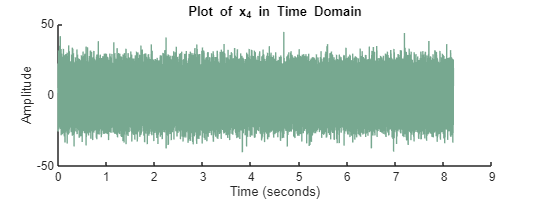
\includegraphics[width=0.5\linewidth]{figures/x4.png}
    \caption{Signal $x_4$ over Time}
    \label{fig:x4}
\end{figure}

The frequency spectrum in Figure \ref{fig:X4} similarly shows that a large amount of noise has been added to the signal.  

\begin{figure}[H]
    \centering
    \includegraphics[width=0.5\linewidth]{figures/X4.png}
    \caption{Frequency Spectrum of Signal $x_4$}
    \label{fig:X4}
\end{figure}


However, notice that the noise appears to begin just before $1000 \unit{Hz}$, as can be seen in Figure \ref{fig:X4_1000}.  This will enable us to extract the majority of the information in the original audio signal, as a large portion of the speech range of frequencies has been preserved.


\begin{figure}[H]
    \centering
    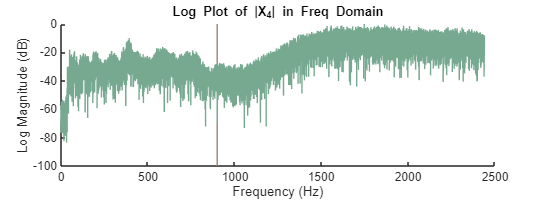
\includegraphics[width=0.5\linewidth]{figures/X4_1000.png}
    \caption{Frequency Spectrum of Signal $x_4$, focused on Audible Frequencies}
    \label{fig:X4_1000}
\end{figure}

In order to filter out the noise that is overpowering the audio, we will use a low pass filter.  Also, because preserving linear phase is important, we will use an FIR filter.  First, we will try to decipher the message, allowing our order to be higher.  After several iterations, we arrive at the design for Filter 1.  The parameters for Filter 1 can be seen in Table \ref{tab:x4_v22}.  The equiripple method yields the best magnitude response for a given order.

\begin{table}[H]
    \centering
    \begin{tabular}{c|cccc}
         Order & Fpass & Fstop & Apass & Astop \\ \hline
         56 & $800  \unit{Hz}$ & $2000  \unit{Hz}$ & $1  \unit{dB} $ & $100  \unit{dB}$
    \end{tabular}
    \caption{Parameters for Filter 1 for Signal $x_4$}
    \label{tab:x4_v22}
\end{table}

Applying the filter to the signal yields the following time and frequency responses in Figure \ref{fig:x4_v22_both}.


\begin{figure}
    \centering
    \includegraphics[width=0.5\linewidth]{figures/x4_v22.png}
    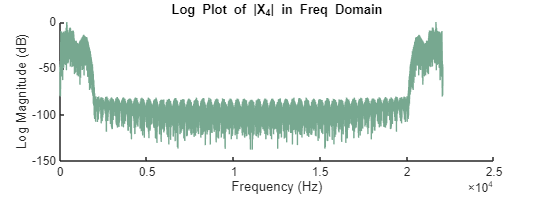
\includegraphics[width=0.5\linewidth]{figures/X4_v22.png}
    \caption{Response of Signal $x_4$ to Filter 1, Order 56}
    \label{fig:x4_v22_both}
\end{figure}

This removes all of the noise, but also removes portions of the speech information.  Despite this, we are still able to interpret the information.  At first, I was only able to hear, ``huh, what is that the light... crush your enemies... it is given before you... and walalalalalanight." Putting this into a google search brought me to a Reddit page quoting Conan the Barbarian.  I followed this lead, and came across a YouTube video that contains the full quote, ``Conan, what is best in life? To crush your enemies, see them driven before you, and to hear the lamentations of their women."  While still distorted, it is easy to hear the words once they are known.  This audio can be heard in the \code{x4\_goodAudio.wav} file in the \href{https://github.com/dbcometto/ece434_cpx2}{GitHub repository}.

Pushing this idea to its maximum, progressively adjusting the parameters enabled lowering the order of the filter to order 5.  The specifications for Filter 2 can be seen in Table \ref{tab:x4_v21}. 

\begin{table}[H]
    \centering
    \begin{tabular}{c|cccc}
         Order & Fpass & Fstop & Apass & Astop \\ \hline
         5 & $100  \unit{Hz}$ & $3300  \unit{Hz}$ & $4  \unit{dB} $ & $39  \unit{dB}$
    \end{tabular}
    \caption{Parameters for Filter 2 for Signal $x_4$}
    \label{tab:x4_v21}
\end{table}

Applying Filter 2 to the signal yields the time and frequency response in Figure \ref{fig:x4_v21_both}.

\begin{figure}[H]
    \centering
    \includegraphics[width=0.5\linewidth]{figures/x4_v21.png}
    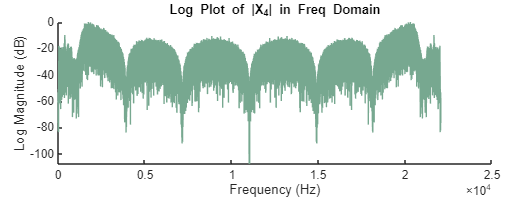
\includegraphics[width=0.5\linewidth]{figures/X4_v21.png}
    \caption{Response of Signal $x_4$ to Filter 2, Order 5}
    \label{fig:x4_v21_both}
\end{figure}

This yields quiet audio with a lot of hissing noise on top.  However, it is still easy to make out the words.  In many ways, the audio sounds better: it had less of the audio information removed.  The audio is just less uncovered.  This response can be heard in the \code{x4\_barelyAudible.wav} file in the \href{https://github.com/dbcometto/ece434_cpx2}{GitHub repository}.


